\documentclass{article}
\usepackage{graphicx} 
\usepackage{hyperref}
\usepackage{adjustbox}
\usepackage{listings}
\usepackage{xcolor}
\usepackage{tabularx} 
\usepackage{booktabs} 
\usepackage{rotating}
\usepackage{csquotes}
\usepackage[
backend=biber,
style=alphabetic,
sorting=ynt,
natbib=true
]{biblatex}

\addbibresource{references.bib}

\lstset{
    basicstyle=\ttfamily\scriptsize,
    breaklines=true,
    frame=single,
    backgroundcolor=\color{gray!5},
    xleftmargin=-1.5cm,
    xrightmargin=-1.5cm
}

\hypersetup{
    colorlinks=true,
    linkcolor=blue,
    urlcolor=cyan
}

\newcommand{\ExoMinerPipeline}{\texttt{ExoMiner Pipeline}}


\title{
    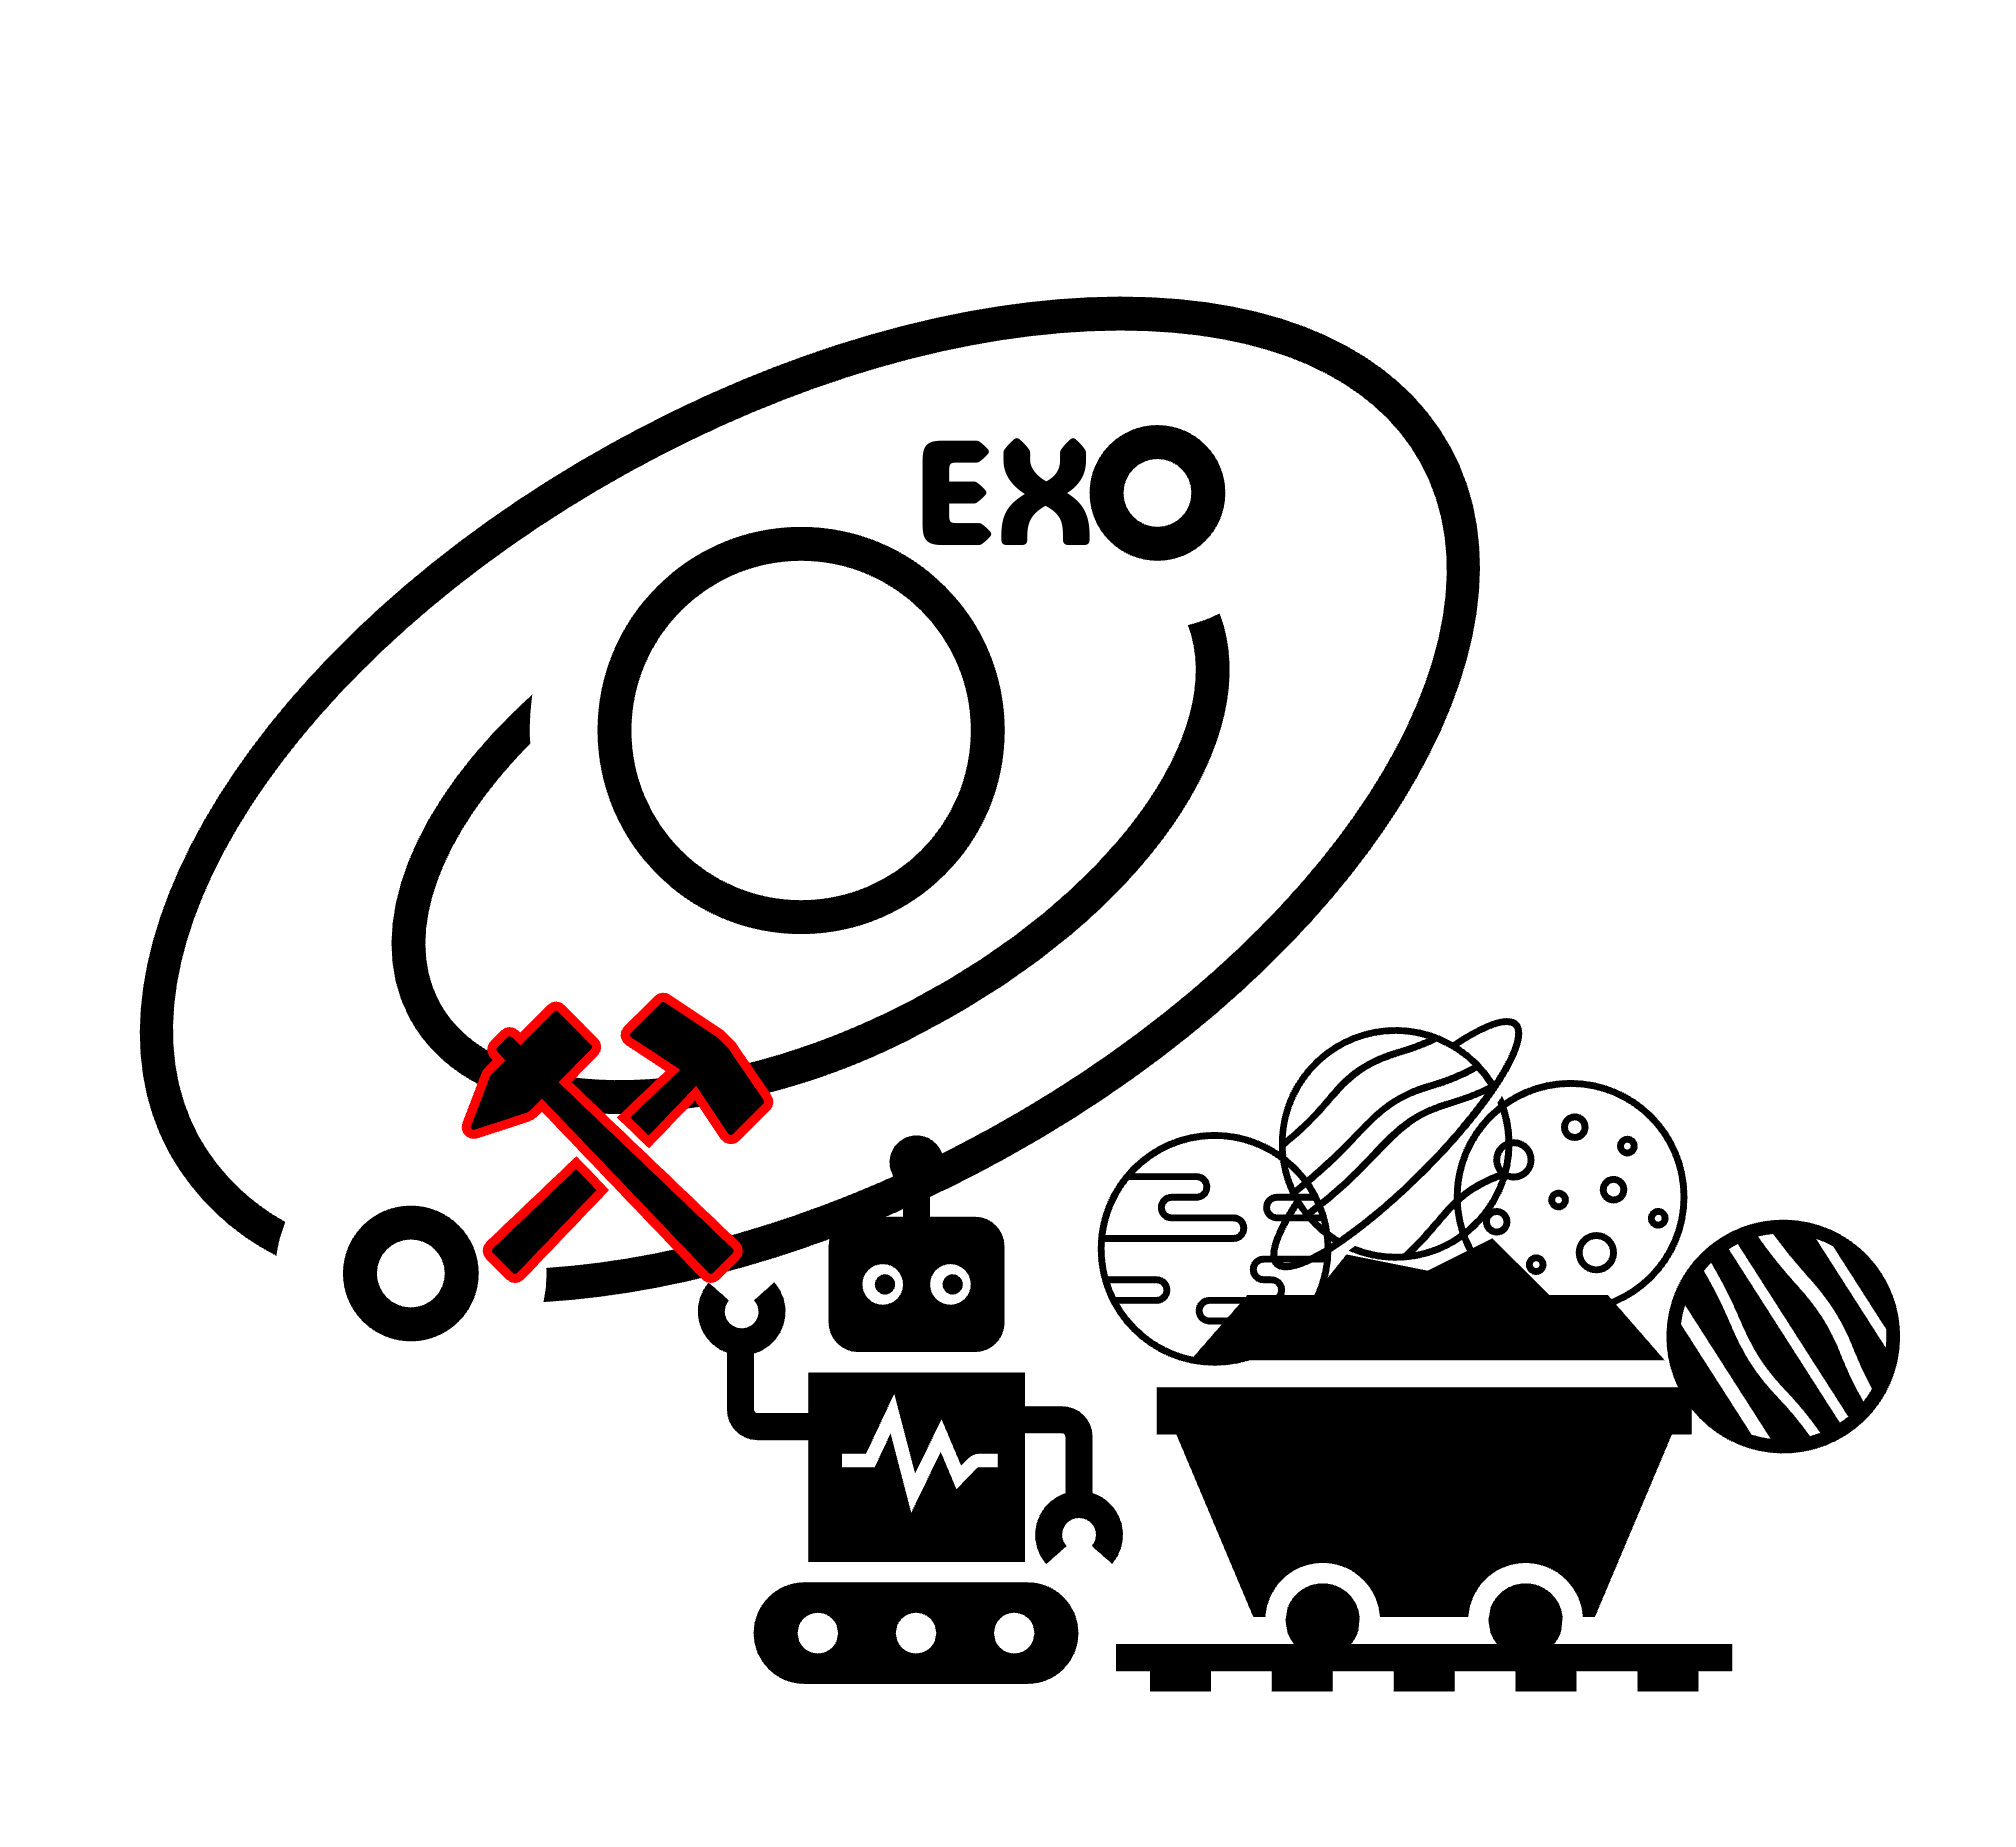
\includegraphics[width=0.35\textwidth]{images/exominer_logo.png} \\
    \vspace{0.5cm}
    ExoMiner Pipeline Outputs \\
    \large For Pipeline Version 2.1
    }
\author{
Miguel Martinho \\\ 
\href{mailto:miguel.martinho@nasa.gov}{miguel.martinho@nasa.gov} \\\ 
Data Sciences Group, Intelligent Systems Division (Code TI) \\
NASA Ames Research Center
}
\date{August 2026}

\begin{document}

\maketitle

\tableofcontents
\newpage 

\section{Introduction}

The \href{https://github.com/nasa/Exominer/tree/main}{\ExoMinerPipeline} was designed as an end-to-end pipeline to aid Subject Matter Experts (SMEs) in the vetting and validation of planet candidates from the TESS Mission. Figure~\ref{fig:exominer_flowchart} describes the pipeline and overall steps from queried TIC IDs to prediction results output for the SPOC TCEs detected for those targets. For a comprehensive documentation on downloading, installing, and using this pipeline, please refer to the documentation guide within the project's official NASA GitHub repository \citep{exominer_github}. This document is intended to describe the outputs of this pipeline for anyone interested in using the pipeline results towards exoplanet candidate vetting. 

\begin{figure}[htbp]
    \centering
    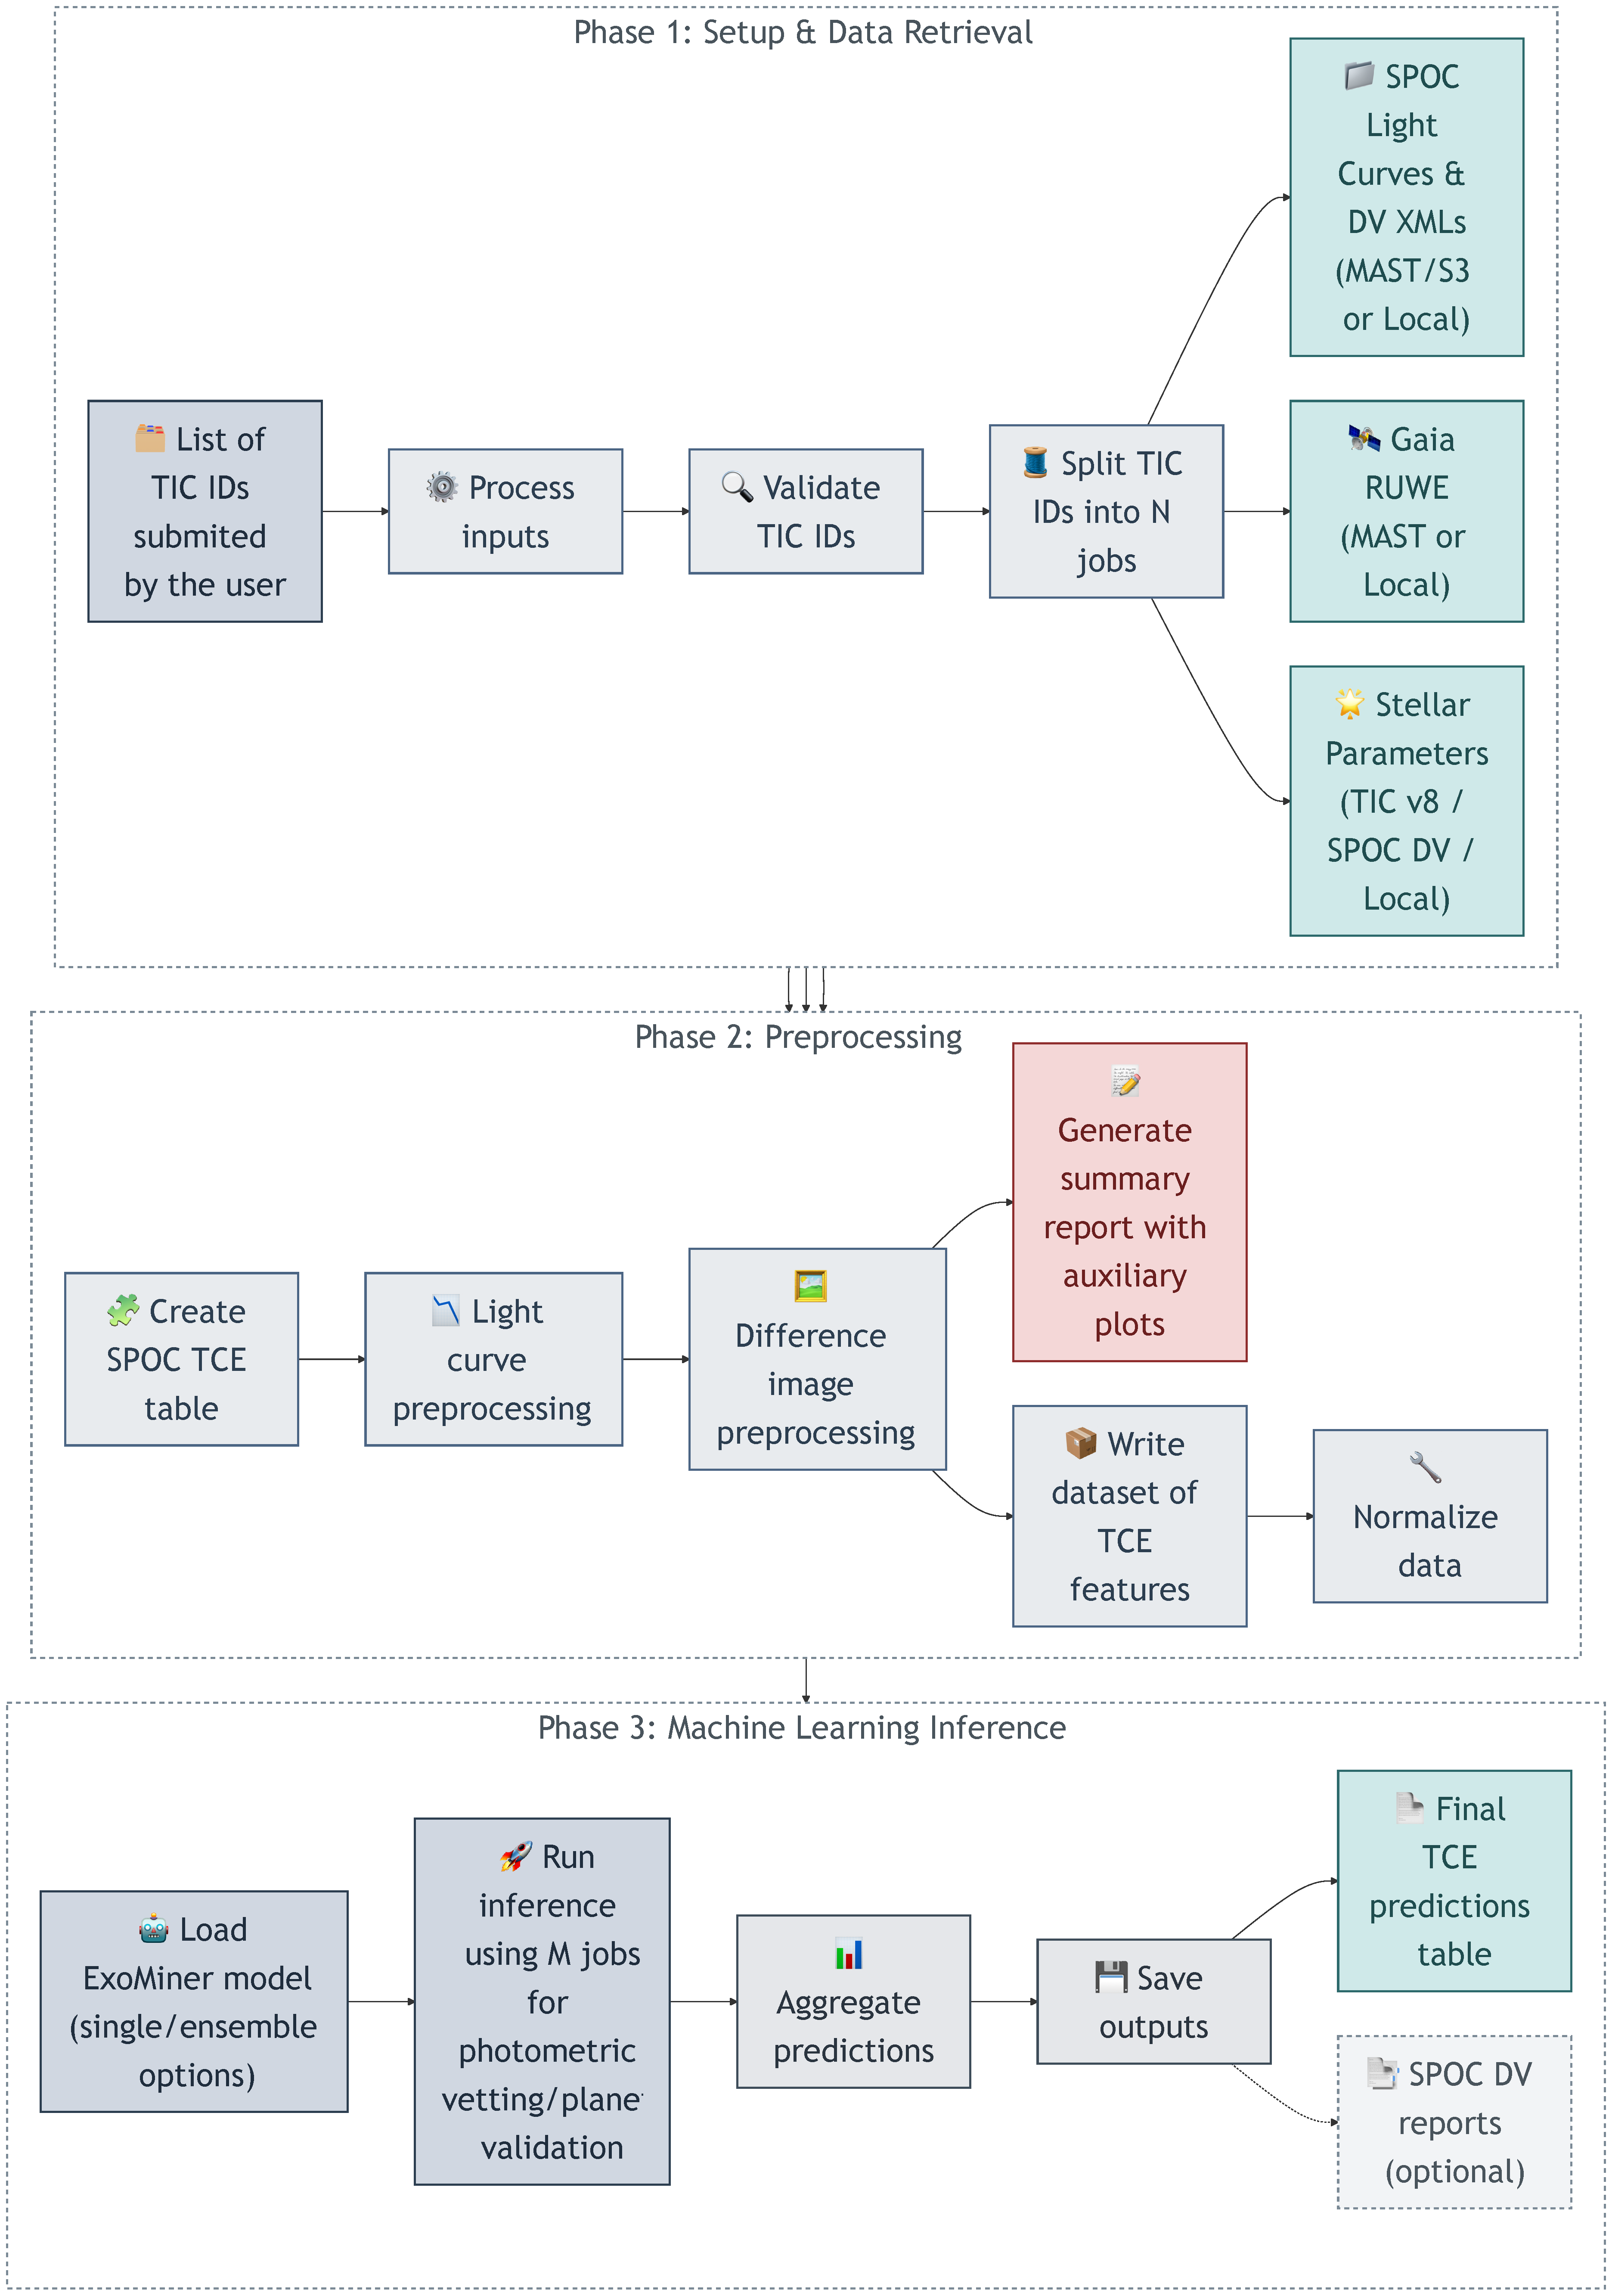
\includegraphics[height=0.90\textheight]{images/exominer-pipeline-flowchart_final.pdf}
    \caption{\ExoMinerPipeline\ flowchart.}
    \label{fig:exominer_flowchart}
\end{figure}

The \ExoMinerPipeline\ generates two main products: a prediction table containing the prediction scores for the SPOC TCEs detected in the set of queried TIC IDs and corresponding sector runs; additionally, a summary report can be optionally generated for each TCE, and includes relevant diagnostic plots that show how the data were preprocessed and ingested by the model to produce the aforementioned prediction scores.

\section{Prediction Table}

The prediction table is the final product generated by the \ExoMinerPipeline. It is exported as a comma-separated values (CSV) file containing two main sections: a metadata header and the tabular prediction data.

\subsubsection*{Metadata Header}
The file begins with a metadata header, denoted by lines starting with the \texttt{\#} character, which serves to preserve run provenance and configuration details. Key information captured in this header includes:
\begin{itemize}
    \item \textbf{Pipeline Versioning:} Git commit hash, build date, and version number (e.g., Version 2.1).
    \item \textbf{Run Configuration:} ExoMiner model used (e.g., \texttt{phot-vetting}), data collection mode (e.g., 2min), and the data sources utilized for stellar parameters and RUWE.
    \item \textbf{Classification Threshold \& Label Map:} Definitions for the target classes, which in the case of photometric vetting include Planet Candidate (PC), Astrophysical False Positive (AFP), and Non-Transiting Phenomena (NTP); for the planet validation task, those classes become Planet and Non-Planet. Each TCE is assigned the disposition of the class that scored the highest as long this score is above the classification threshold.
\end{itemize}

\subsubsection*{Data Columns}
Following the metadata header, the file provides the model's predictions for each evaluated TCE. The tabular data columns are defined in Table~\ref{tab:data_columns}.

\begin{table}[htbp]
    \centering
    \caption{Description of the data columns provided in the \ExoMinerPipeline\ prediction table output.}
    \label{tab:data_columns}
    \renewcommand{\arraystretch}{1.4} 
    \begin{tabularx}{\textwidth}{@{} l X @{}}
        \toprule
        \textbf{Column Name} & \textbf{Description} \\
        \midrule
        \texttt{uid} & Unique SPOC TCE identifier formatted with the pattern \texttt{<tic\_id>-}\allowbreak\texttt{<tce\_plnt\_num>-}\allowbreak\texttt{S<sector\_run\_id>} (e.g., \texttt{1942969-1-S14-86}). \\
        \texttt{target\_id} & TIC ID of the target star (integer scalar). \\
        \texttt{sector\_run} & SPOC sector run identifier. Represented as a single sector or a multi-sector range (e.g., \texttt{14-86}). \\
        \texttt{tce\_plnt\_num} & SPOC TCE planet number (integer scalar). \\
        \texttt{tce\_period} & TCE period in days (float scalar). \\
        \texttt{tce\_duration} & TCE transit duration in hours (float scalar). \\
        \texttt{tce\_time0bk} & TCE time of first transit in BTJD (float scalar). \\
        \texttt{tce\_depth} & TCE transit depth in parts per million (ppm). \\
        \texttt{ruwe} & Renormalized Unit Weight Error from Gaia (float scalar). \\
        \texttt{tce\_prad} & TCE planet radius in Earth radii (float scalar). \\
        \texttt{tce\_max\_mult\_ev} & TCE maximum multiple event statistic (float scalar). \\
        \texttt{matchedToiId} & Matched TOI ID from the SPOC Data Validation (DV) report (e.g., \texttt{5459.01}), or \texttt{not\_matched} if no match is found. \\
        \texttt{score\_<disp>} & The ExoMiner mean score for the respective disposition class. When using the photometric vetting model, these three class probabilities sum to 1. If using the planet vs. non-planet validation model, there is a single score for the planet class. \\
        \texttt{score\_std\_<disp>} & The ExoMiner standard deviation score for each class. \\
        \texttt{prediction} & The final predicted disposition assigned by the pipeline, based on the classification threshold and the ExoMiner mean score. \\
        \bottomrule
    \end{tabularx}
\end{table}

\subsubsection*{Example Output}
Figure~\ref{fig:csv_snippet} provides an example of the raw CSV output generated by the \ExoMinerPipeline, showing the header and two evaluated TCEs.

\begin{figure}[htbp]
\begin{lstlisting}
# Run: exominer-pipeline-run_tess-spoc-2min_s14-s86_test-deliver-poc_6-15-2026_0833
# Created: 2026-06-15T20:15:37.934131
# Version Number: 2.1
# Git Commit Hash: 9ee77fde310cef20b470888ee5392a2887b77fc4
# Build Date: 6-9-2026
# ExoMiner Model: phot-vetting
# Label Map: {'PC': 1, 'AFP': 2, 'NTP': 0}
# Data Collection Mode: 2min
# Stellar Parameters Source: ticv8
# RUWE Source: gaiadr2
# Classification Threshold: 0
# Disposition Definitions: ========================
# PC: planet candidate
# AFP: astrophysical false positive
# NTP: non-transiting phenomena
# Column Definitions: ========================
# Column: uid: Unique SPOC TCE identifier with pattern <tic_id>-<tce_plnt_num>-S<sector_run_id> (e.g., 123456789-1-S1, 123456789-1-S1-3) (string)
# Column: target_id: TIC ID of the target star (int scalar)
# Column: sector_run: SPOC sector run identifier. If single sector run follows format <sector>. If multisector runs follows format <start_sector>-<end_sector>(string)
# Column: tce_plnt_num: SPOC TCE planet number (int scalar)
# Column: tce_period: TCE period in days (float scalar)
# Column: tce_duration: TCE duration in hours (float scalar)
# Column: tce_time0bk: TCE time of first transit in BTJD (float scalar)
# Column: tce_depth: TCE depth in ppm (float scalar)
# Column: ruwe: Renormalized Unit Weight Error from Gaia (float scalar)
# Column: tce_prad: TCE planet radius in Earth radii (float scalar)
# Column: tce_max_mult_ev: TCE max multiple event statistic (float scalar)
# Column: matchedToiId: matched TOI ID from SPOC DV (e.g., "1234.01" or "not_matched" if no match found) (string)
# Column: score/score_<disp>: if using ExoMiner for photometric vetting there are three columns with ExoMiner mean scores for PC/AFP/NTP classes/disposition categories summing up to 1. For planet vs not-planet validation there is a single score.
# Column: prediction: predicted disposition based on classification threshold and ExoMiner mean score(s)
uid, target_id, sector_run, tce_plnt_num, tce_period, tce_duration, tce_time0bk, tce_depth, ruwe, tce_prad, tce_max_mult_ev, matchedToiId, score_PC, score_AFP, score_NTP, prediction
1942969-1-S14-86, 1942969, 14-86, 1, 2.80783, 1242.478, 2912.802, 6449.58, 0.813, 18.841, 18.745, 5459.01, 0.987, 0.011, 0.0001, PC
2006984-1-S14-86, 2006984, 14-86, 1, 92.5468, 1410.636, 1906.988, 376.064, 0.790, 33.392, 9.002, not_matched, 0.0003, 0.007, 0.992, NTP
\end{lstlisting}
\caption{Snippet of the \ExoMinerPipeline\ prediction table output (CSV format). Float values have been truncated for display purposes.}
\label{fig:csv_snippet}
\end{figure}

\section{Summary Report}

As supporting products, the pipeline can generate a summary report in PDF format for each SPOC TCE detected for the queried TIC IDs. These reports are an optional product generated by the \ExoMinerPipeline\ and they were created to provide:
\begin{itemize}
    \item Outputs at the end of different steps in the data preprocessing pipeline to visualize the input features (e.g., flux time series, difference images) ingested by the model and derive insights about model behavior and how to improve both the data preprocessing pipeline and model architecture to achieve a better performance.
    \item Plots and visualizations similar to those used by SMEs for vetting of planet candidates. The Data Validation reports generated by the SPOC pipeline~\citep{Jenkins2016SPIE} were used as a guideline when designing the summary report provided by the \ExoMinerPipeline, although both contain plots that are not shared.
\end{itemize}

In the following sections, we describe each plot and image shown in the summary report using 2-min SPOC TCE \texttt{TIC 66818296.1} in S1-S92 as an example.

\subsection{Flux and Centroid Offset}

The phase-folded and binned flux and centroid plots~\ref{fig:phase_folded_flux-centroid} show a condensed representation of most of the time series provided as input to the model. The top of the page includes the SPOC TCE's ephemerides along with several TCE fit parameters such as transit depth, MES, and planet radius. All these values are sourced from the SPOC DV results. The set of stellar parameters provided by the source catalog (e.g., TICv8) are also shown. The names in the header follow the nomenclature used in the SPOC pipeline and can be found in the Exoplanet Archive Kepler's TCEs data columns definitions table\citep{nexa_tce_api}. All of these plots were obtained after detrending the corresponding time series (i.e., flux, flux-weighted centroid motion) using a Savizkty-Golay filter and phase-folding it using the detected SPOC TCE's epoch and orbital period. Each time series datum (i.e., black dot) represents the median value within the bin, while the red dashed line shows the bin standard error of the mean envelope. More transit observations as well as cleaner transits will make the envelope tighter. For a more detailed explanation of the data preprocessing steps we refer the reader to~\citep{valizadegan2022exominer,valizadegan2025exominer++}. 

Each plot in this page shows in its title the name of time series and the number of transits that were phase-folded and binned to create it. The x-axis shows the phase in hours centered in the detected epoch, with the \enquote{transit-view} plots showing the phase in $[-2.5,2.5]$ transit durations while the \enquote{full-orbit} plots show the complete orbital period. In the flux time series plots, the y-axis shows the relative flux. For the centroid motion time series, the centroid offset is shown relative to the target's TIC coordinates. In several cases, this absolute distance metric can be unreliable and may differ from the vector displacements reported in standard SPOC centroid offset plots which rely on difference image analysis. This discrepancy arises because the measured center of light often contains a static baseline offset from the catalog position due to background crowding (blending), stellar proper motion, or slight coordinate systematic biases. The \enquote{full-orbit trend} plot shows the phase-folded and binned residual of the Savitzky-Golay filter. As legacy, the momentum dump flag time series is shown as part of this page, although no longer used by ExoMiner as an input feature.

% \begin{figure}[htbp]
%     \centering
%     % Constrain to textwidth so it doesn't bleed off the edges
%     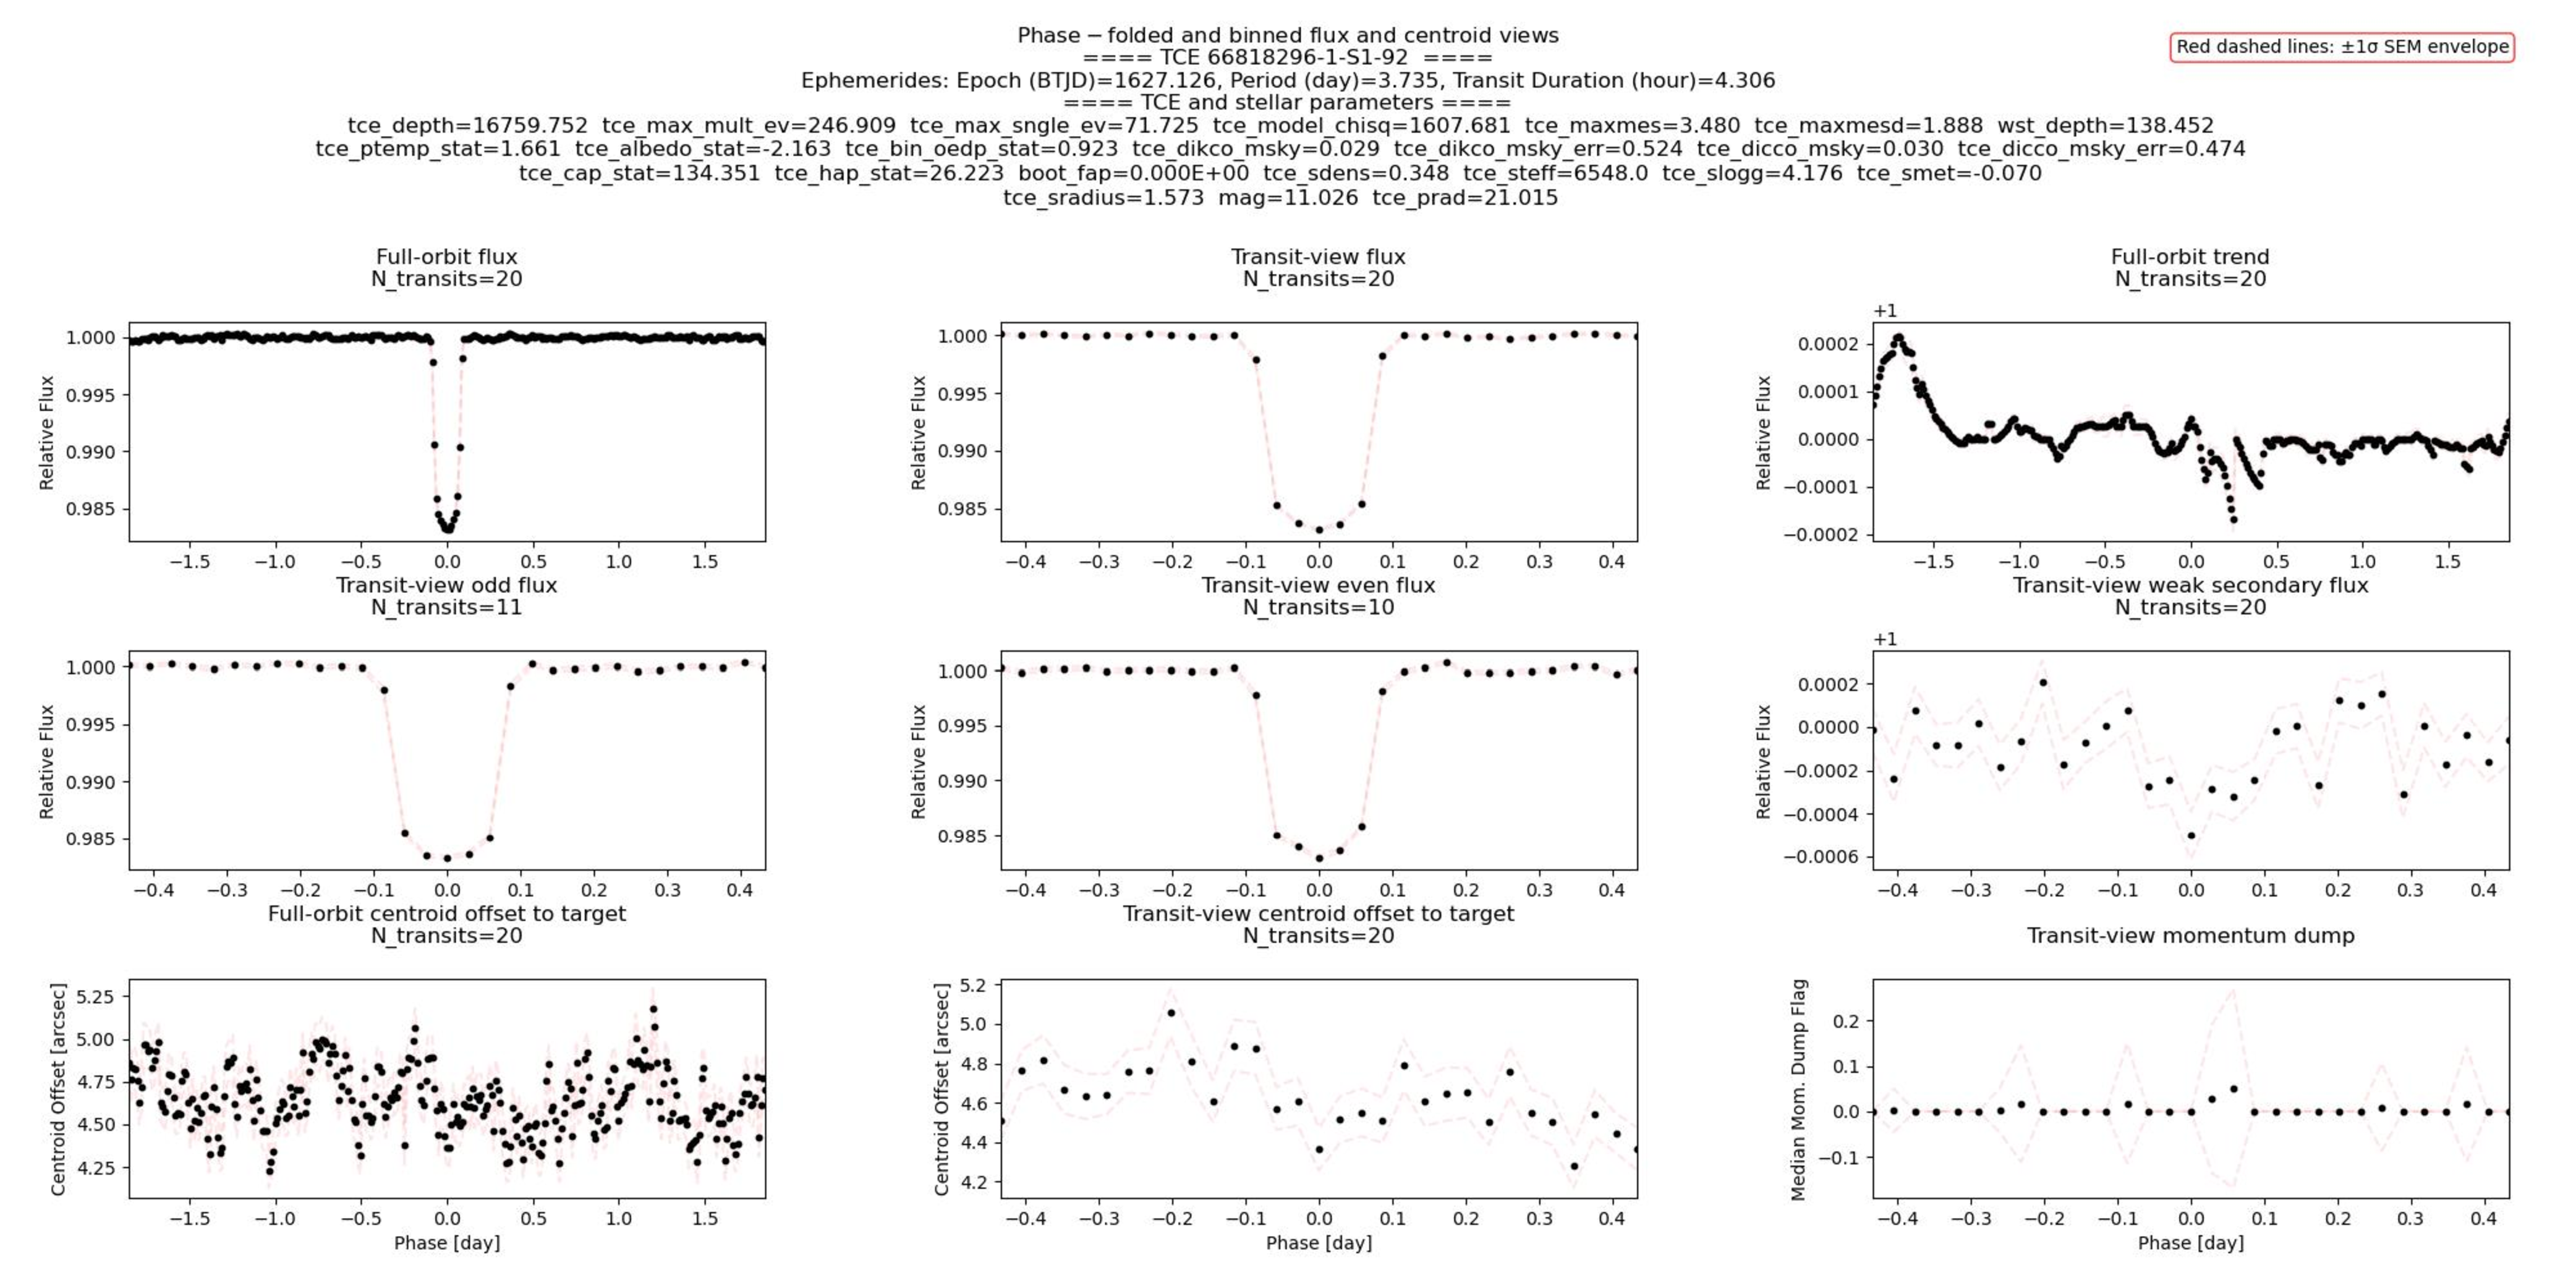
\includegraphics[width=\textwidth]{images/tess-spoc-tce_tic66818296-1-S1-92_summary_exominer-pipeline_phasef-bin-flux-centroid.pdf}
%     \caption{Phase-folded and binned flux and centroid plots for TIC 66818296.1.}
%     \label{fig:phase_folded_flux}
% \end{figure}

\begin{sidewaysfigure}[htbp]
    \centering
    % Because the page is sideways, the 'width' of the image is now matched to the 'height' of the text area!
    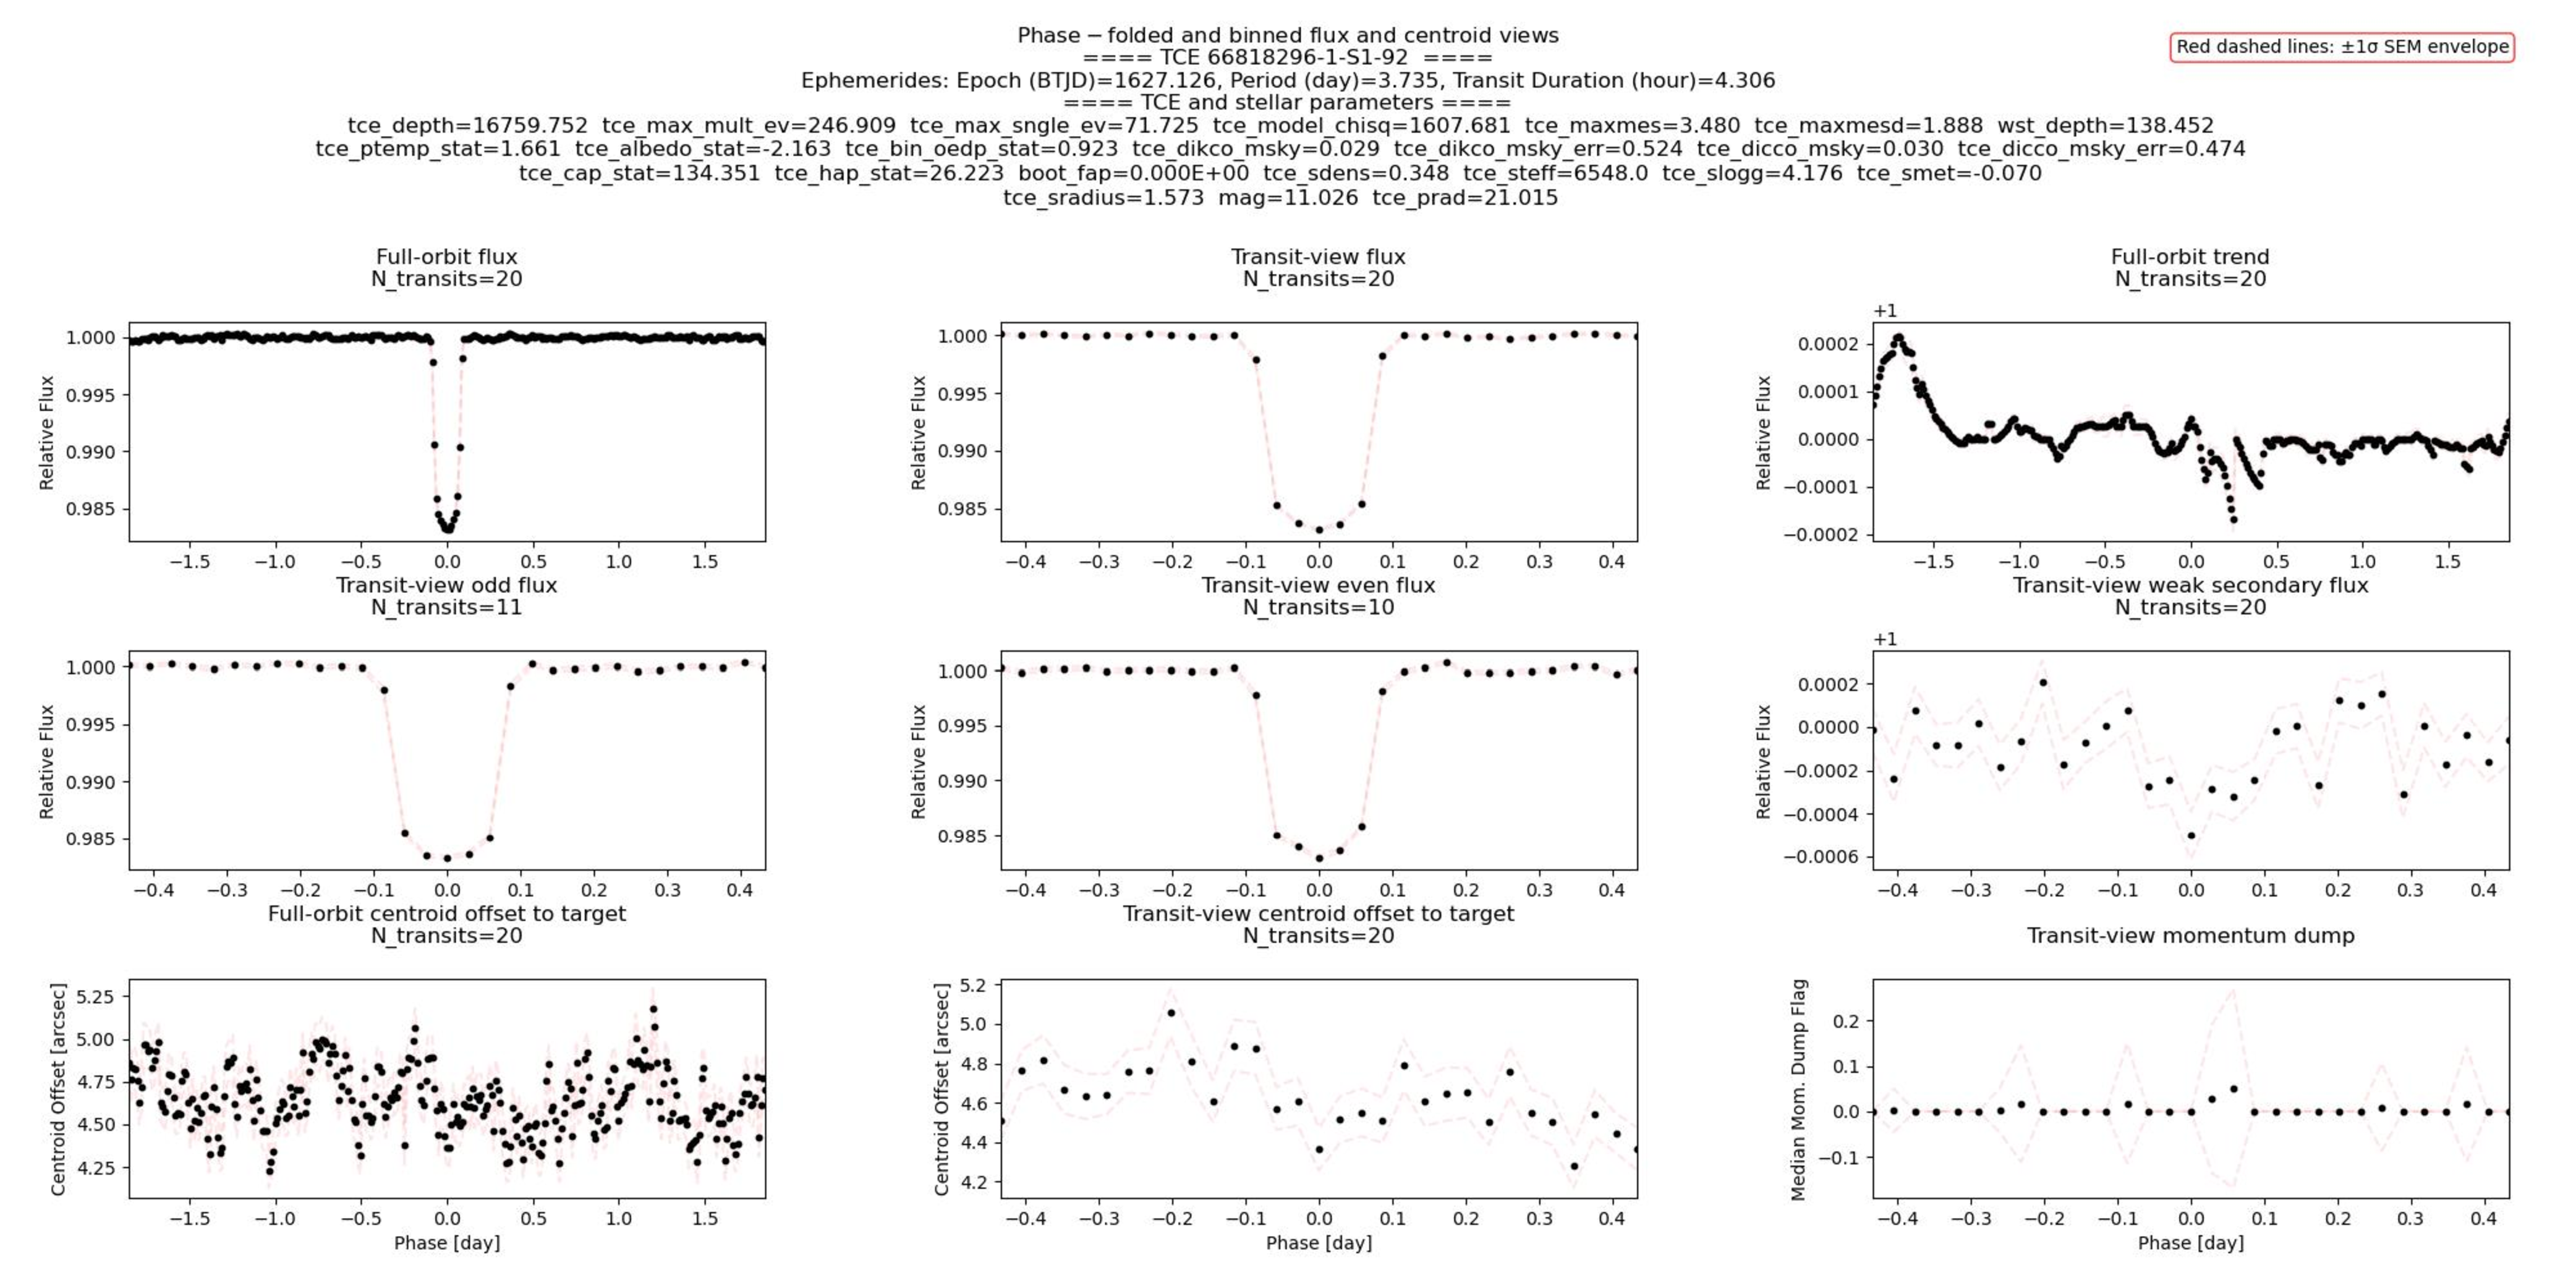
\includegraphics[width=\textheight]{images/tess-spoc-tce_tic66818296-1-S1-92_summary_exominer-pipeline_phasef-bin-flux-centroid.pdf}
    \caption{Phase-folded and binned flux and centroid plots for \texttt{TIC 66818296.1}.}
    \label{fig:phase_folded_flux-centroid}
\end{sidewaysfigure}

\subsection{Weak Secondary}

The weak secondary plots shown in Figure~\ref{fig:weak_secondary} are centered on the detected secondary transit. The top plot shows the phase-folded flux time series and the red dashed vertical line points to the primary transit midpoint. The bottom plots show the \enquote{transit-view} centered also on the secondary transit midpoint and show the phase range in $[-2.5,2.5]$ transit durations. In the bottom-left plot, if the primary transit is within that interval, a red dashed vertical line will indicate its location. Finally, the bottom-right plot shows the same view as the bottom-left counterpart, but without the individual data points and the phase-folded and binned transit-view time series was normalized by the absolute minimum, which makes the differences in magnitude more salient. This is the normalized version that is given as input to the model.

\begin{figure}[htbp]
    \centering
    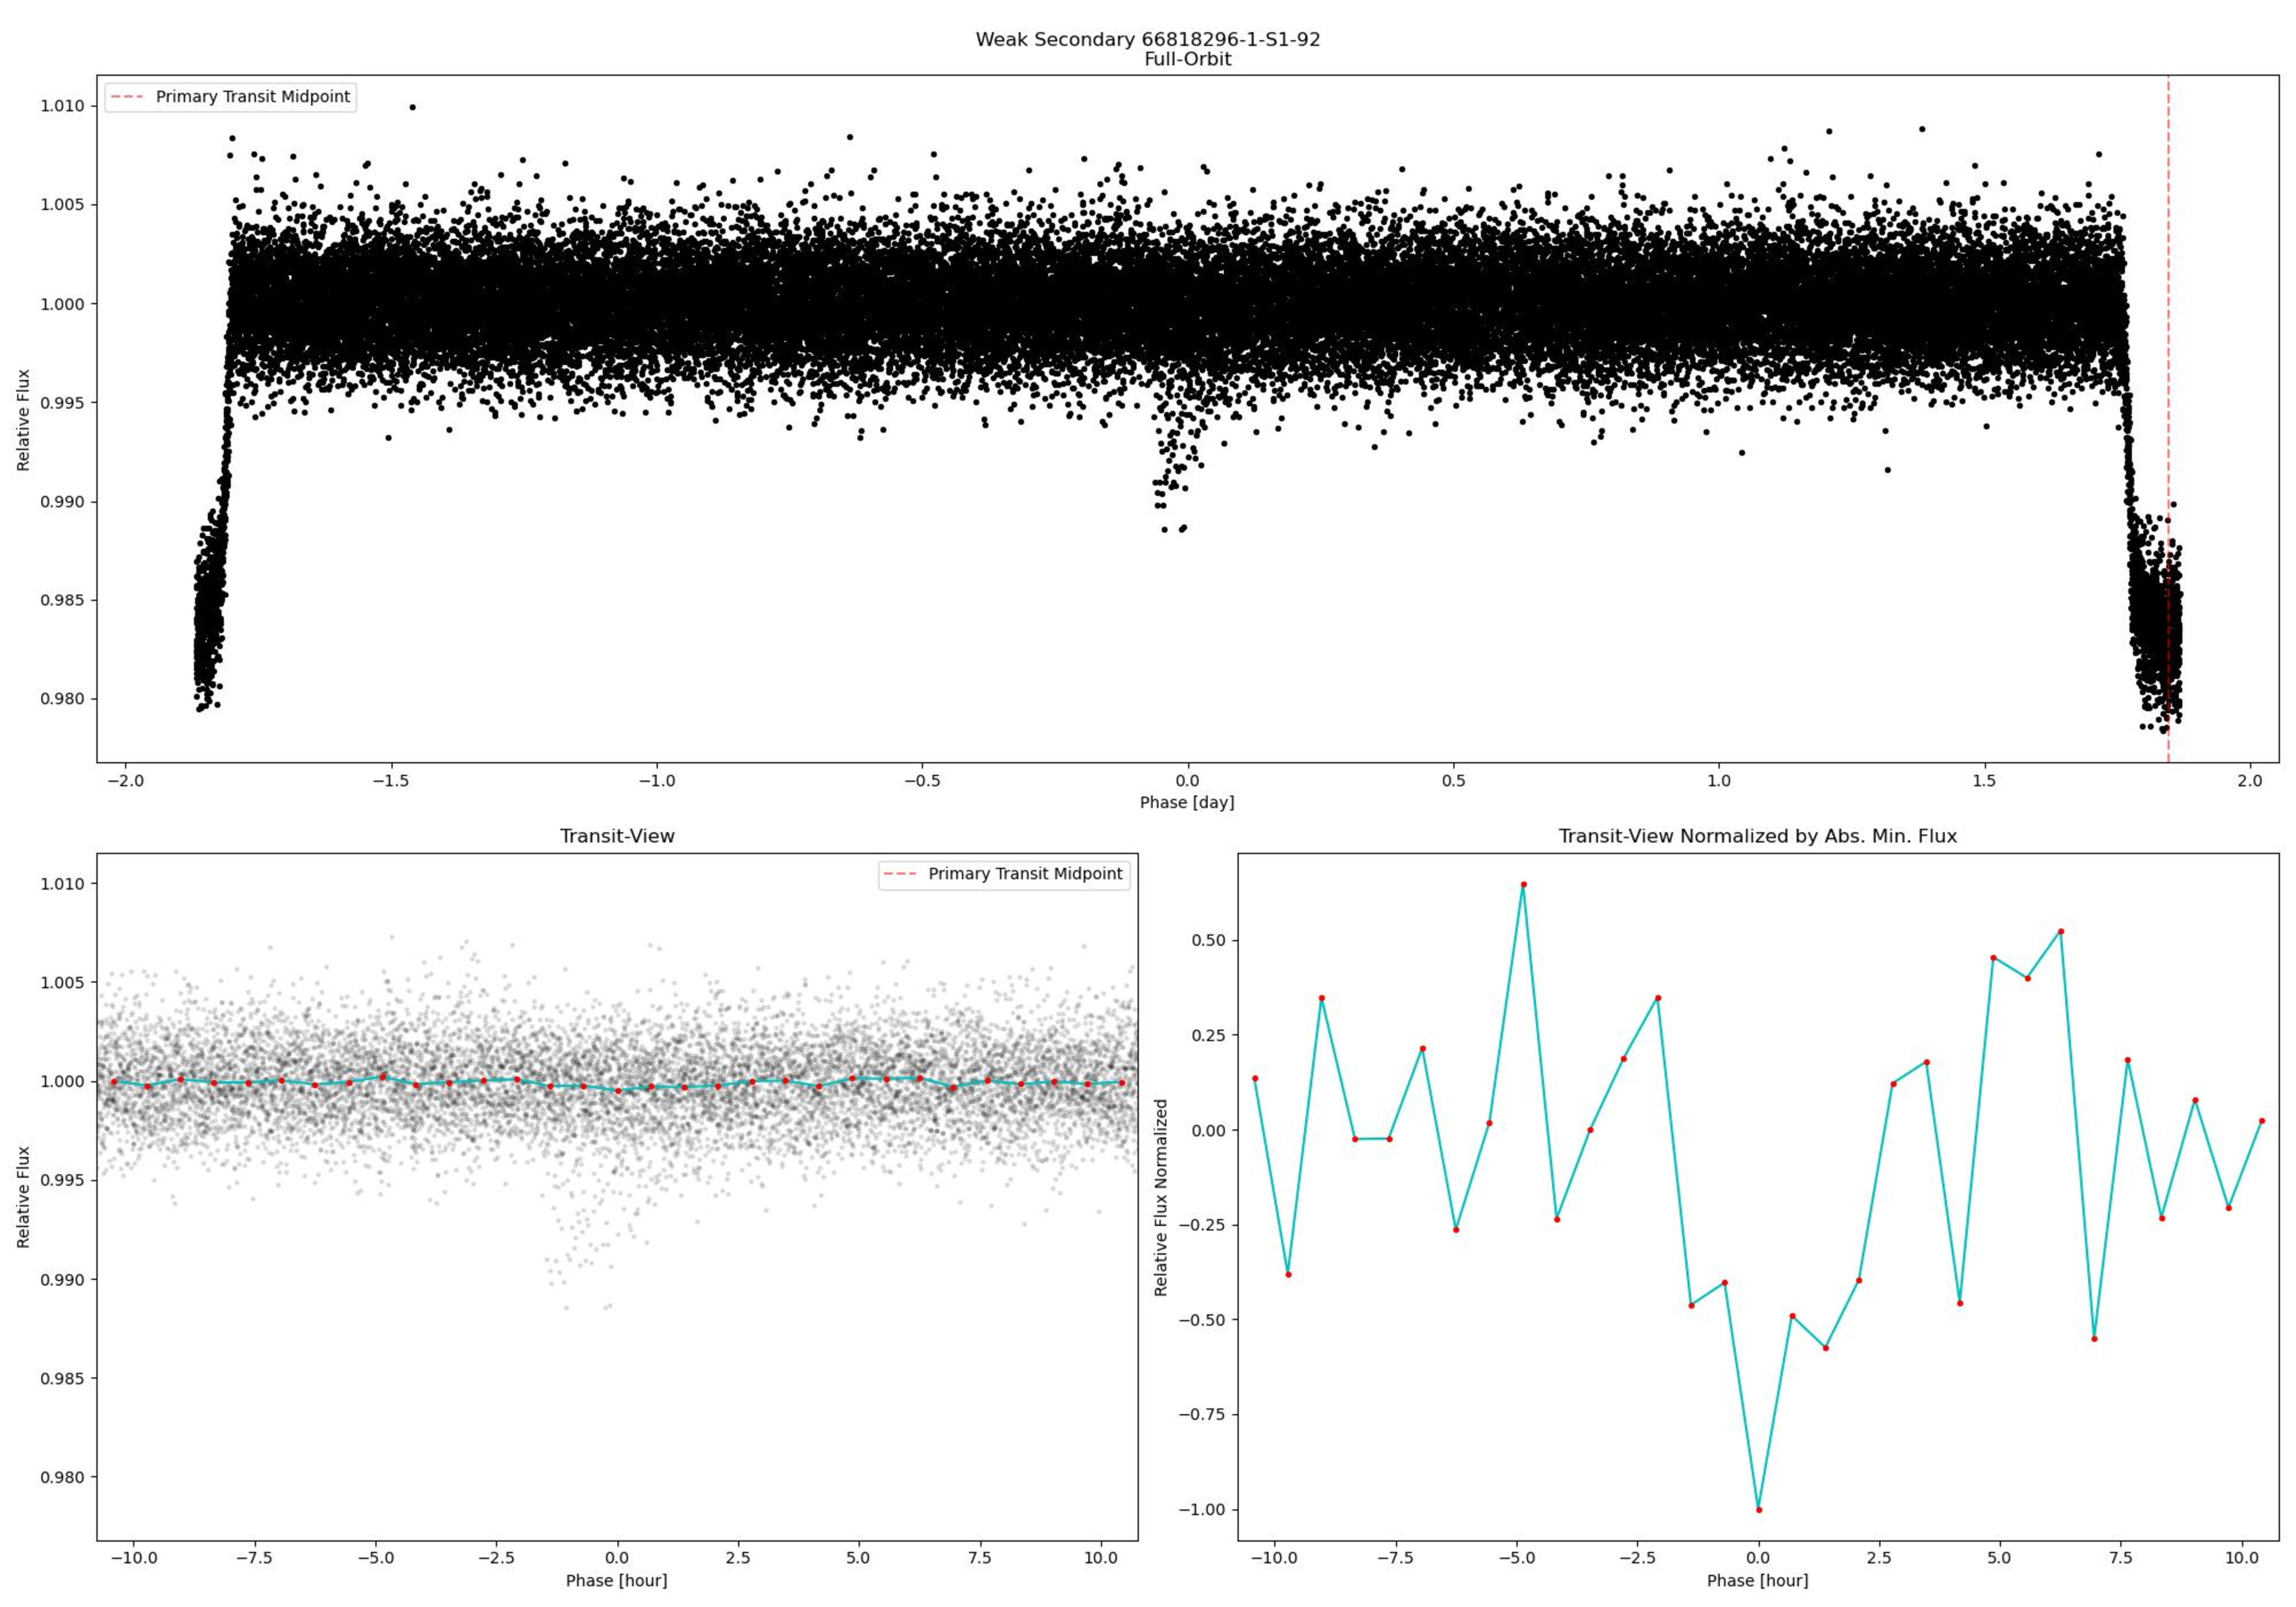
\includegraphics[width=\textwidth]{images/tess-spoc-tce_tic66818296-1-S1-92_summary_exominer-pipeline_weak-secondary.pdf}
    \caption{Weak secondary plots for \texttt{TIC 66818296.1}.}
    \label{fig:weak_secondary}
\end{figure}

\subsection{Odd-even}

For the odd-even transit depth comparison, the plots in the top row of the Figure~\ref{fig:odd_even} show the phase-folded and binned transit-view flux time series for the odd (left) and even (right). The bottom plot overlaps the two binned time series for easier visual comparison. The two time series were created by using the same TCE ephemerides but using alternating phases. The red dots show the median bin values and are connected by lines. The data points used to create the binned versions are shown in black with some transparency.

\begin{figure}[htbp]
    \centering
    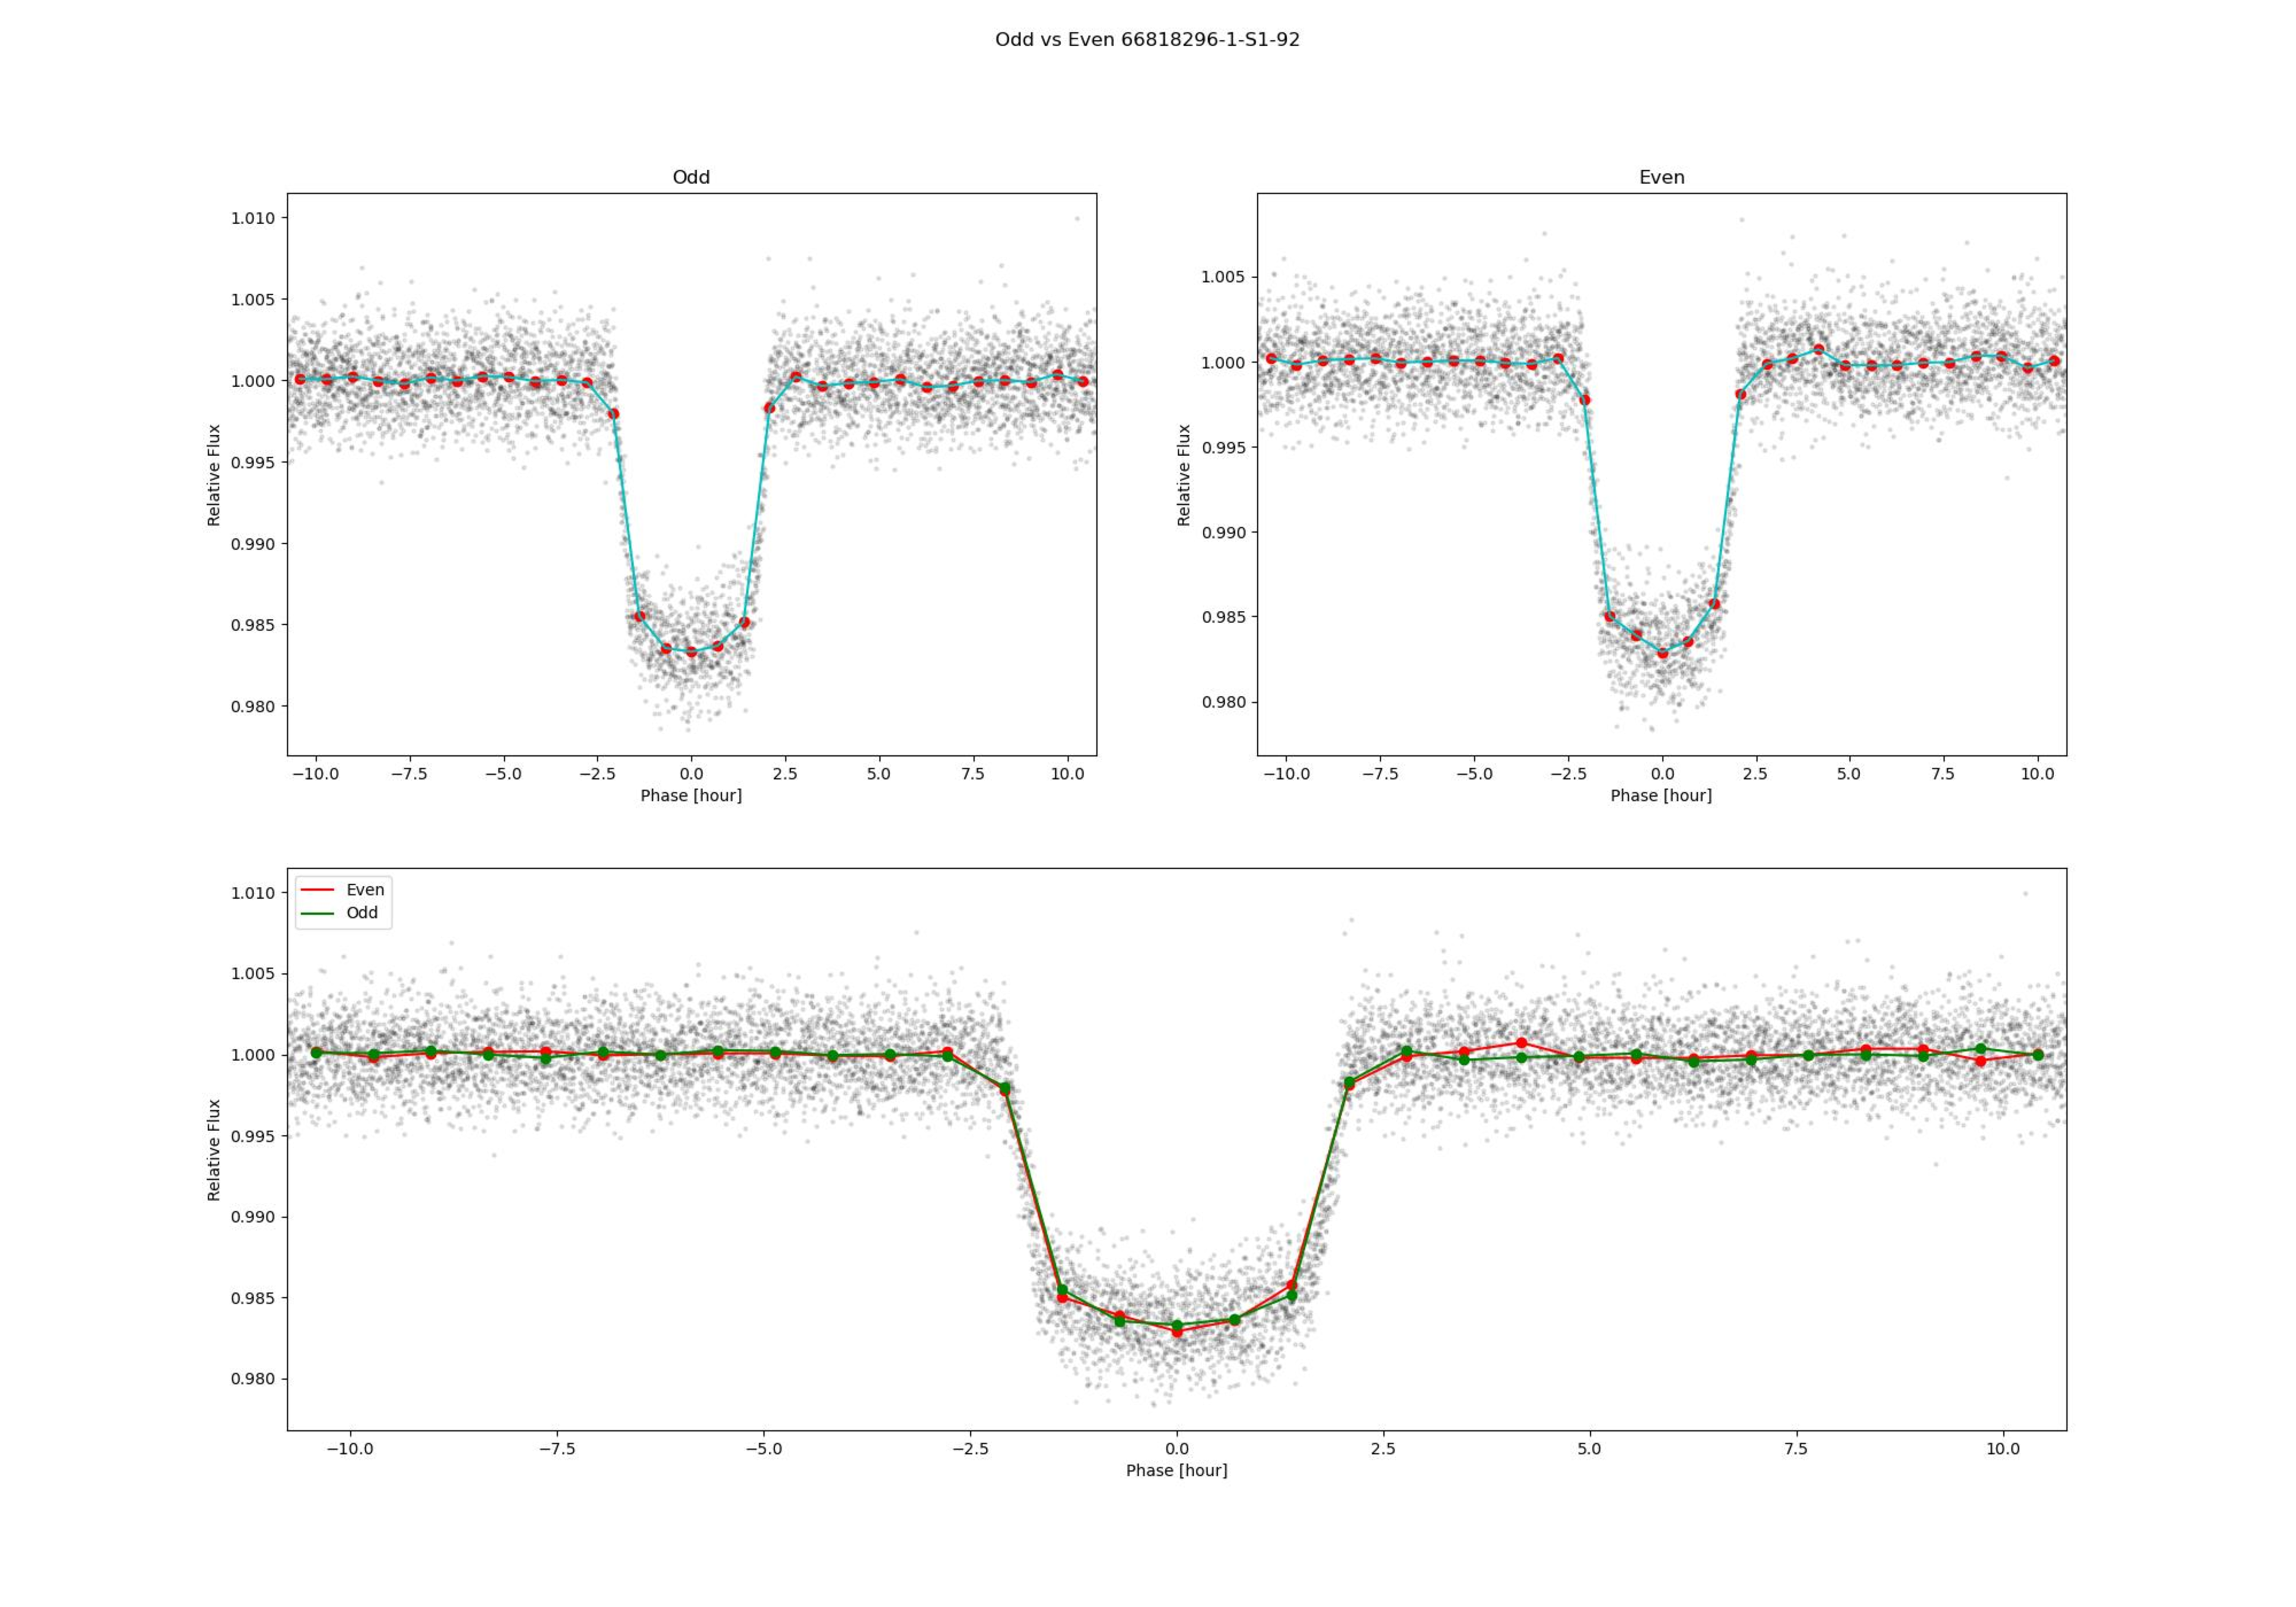
\includegraphics[width=\textwidth]{images/tess-spoc-tce_tic66818296-1-S1-92_summary_exominer-pipeline_odd-even.pdf}
    \caption{Odd-even plots for \texttt{TIC 66818296.1}.}
    \label{fig:odd_even}
\end{figure}

\subsection{Periodogram}

The periodogram page shown in Figure~\ref{fig:pgram} shows the full flux time series in the top plot. For multisector run TCEs whose targets were observed in multiple sectors, this plot can be squashed and hard to read since it spans the full observation time from the first to the last observed sector. The transit pulse model (TPM) time series shows a simple transit pulse created using the detected ephemerides. The figure's header shows the period and corresponding frequency detected by the SPOC pipeline. The center plot shows the periodogram for both the flux and TPM time series. The first five harmonics are highlighted using red dashed vertical lines, and the header shows the max amplitude and its corresponding frequency. Both periodograms are also shown using a smoothed version. The bottom plot shows the same data, but each periodogram was normalized by its maximum amplitude. All periodograms are shown in a log-scale in the frequency domain.

\begin{figure}[htbp]
    \centering
    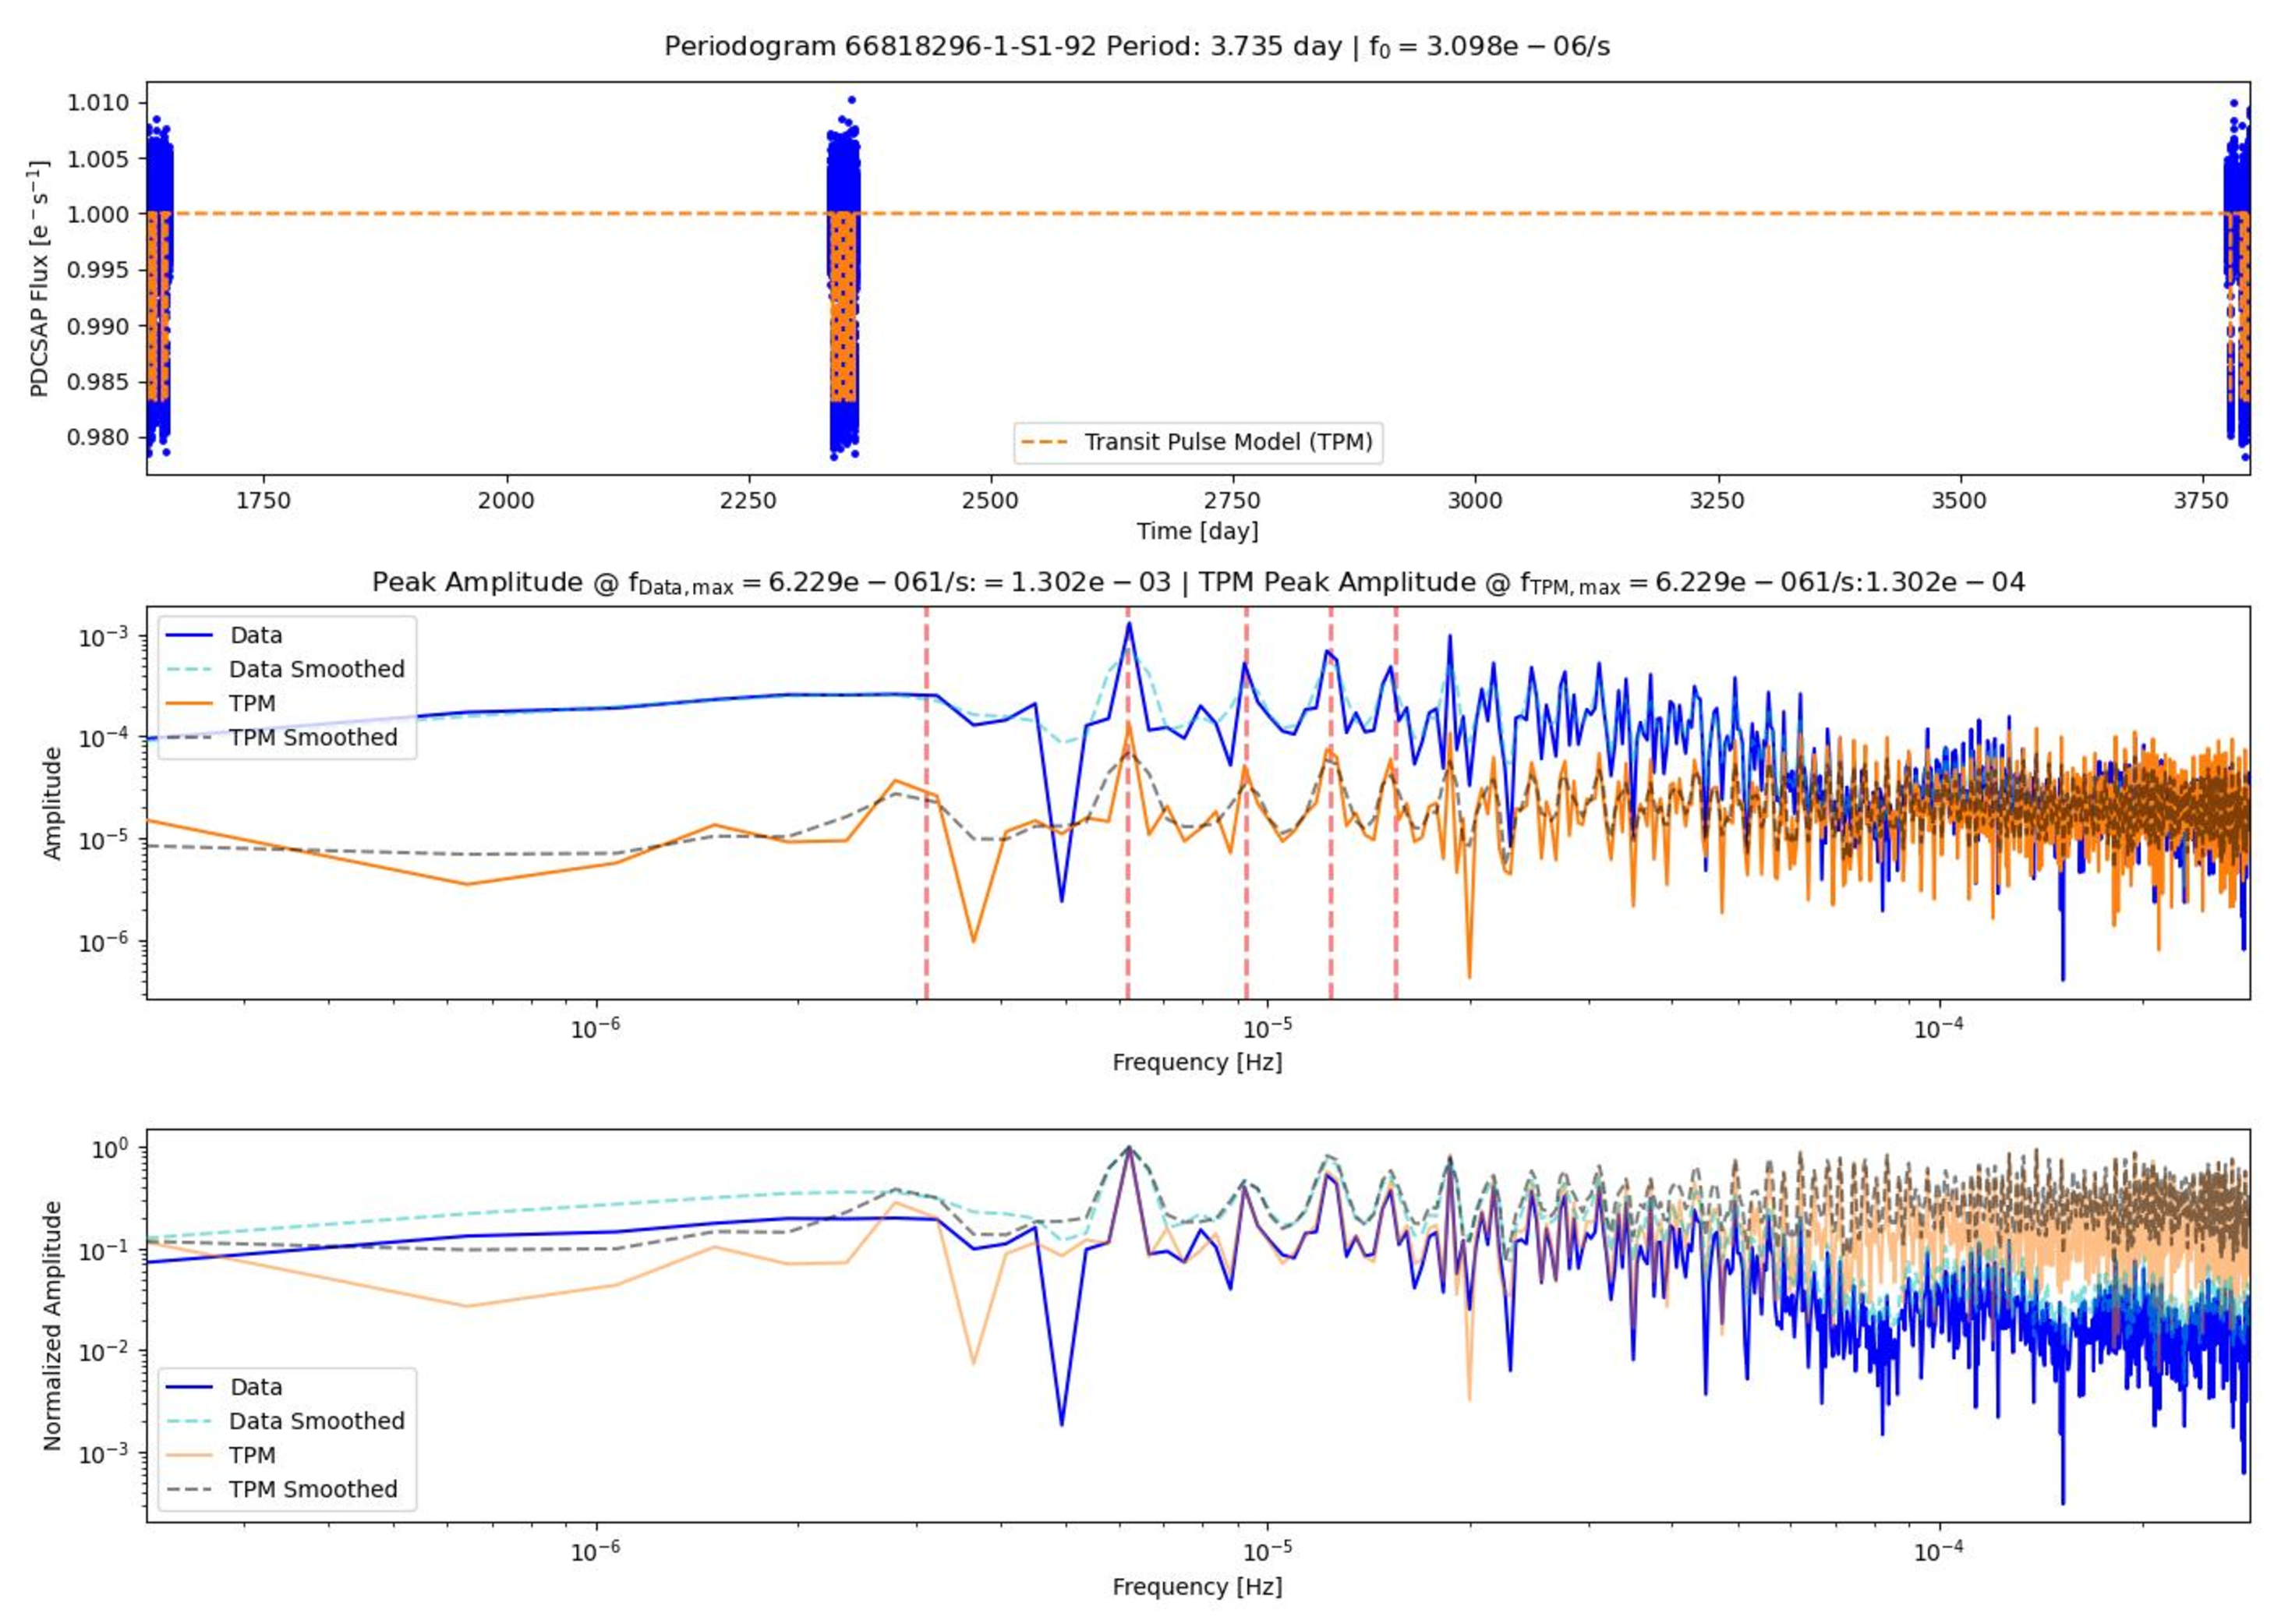
\includegraphics[width=\textwidth]{images/tess-spoc-tce_tic66818296-1-S1-92_summary_exominer-pipeline_pgram.pdf}
    \caption{Periodogram plots for \texttt{TIC 66818296.1}.}
    \label{fig:pgram}
\end{figure}

\subsection{Difference Image}

For each sector the target was observed and it was possible for SPOC to generate difference images for the TCE, the summary report shows a page with several images related to the difference image data in that sector. Figure~\ref{fig:diff_img} shows an example for \texttt{TIC 66818296.1} in sector 12. In all these images the location of the target according to its TIC coordinates is shown as a red cross. The title of the figure shows the sector ID, the target's TESS Magnitude, and the computed quality metric in the SPOC Data Validation (DV) pipeline (correlation between the difference image and the pixel response function centered on the centroid of the difference image). Four different types of images are computed per sector:
\begin{itemize}
    \item Difference flux: mean image created by subtracting the in-transit image from the out-of-transit image. This image is created in the DV module of the SPOC pipeline.
    \item Out-of-transit flux: mean image created using all image data for the out-of-transit cadences. This image is created in the DV module of the SPOC pipeline. Any negative pixels are greyed out.
    \item SNR flux: computed as the difference image flux divided by the uncertainty in each pixel~\cite{Twicken_2018_DV}.
    \item Valid pixels: this is a quality mask that shows which pixels are deemed invalid (e.g., negative out-of-transit image pixels).
\end{itemize}

\begin{figure}[htbp]
    \centering
    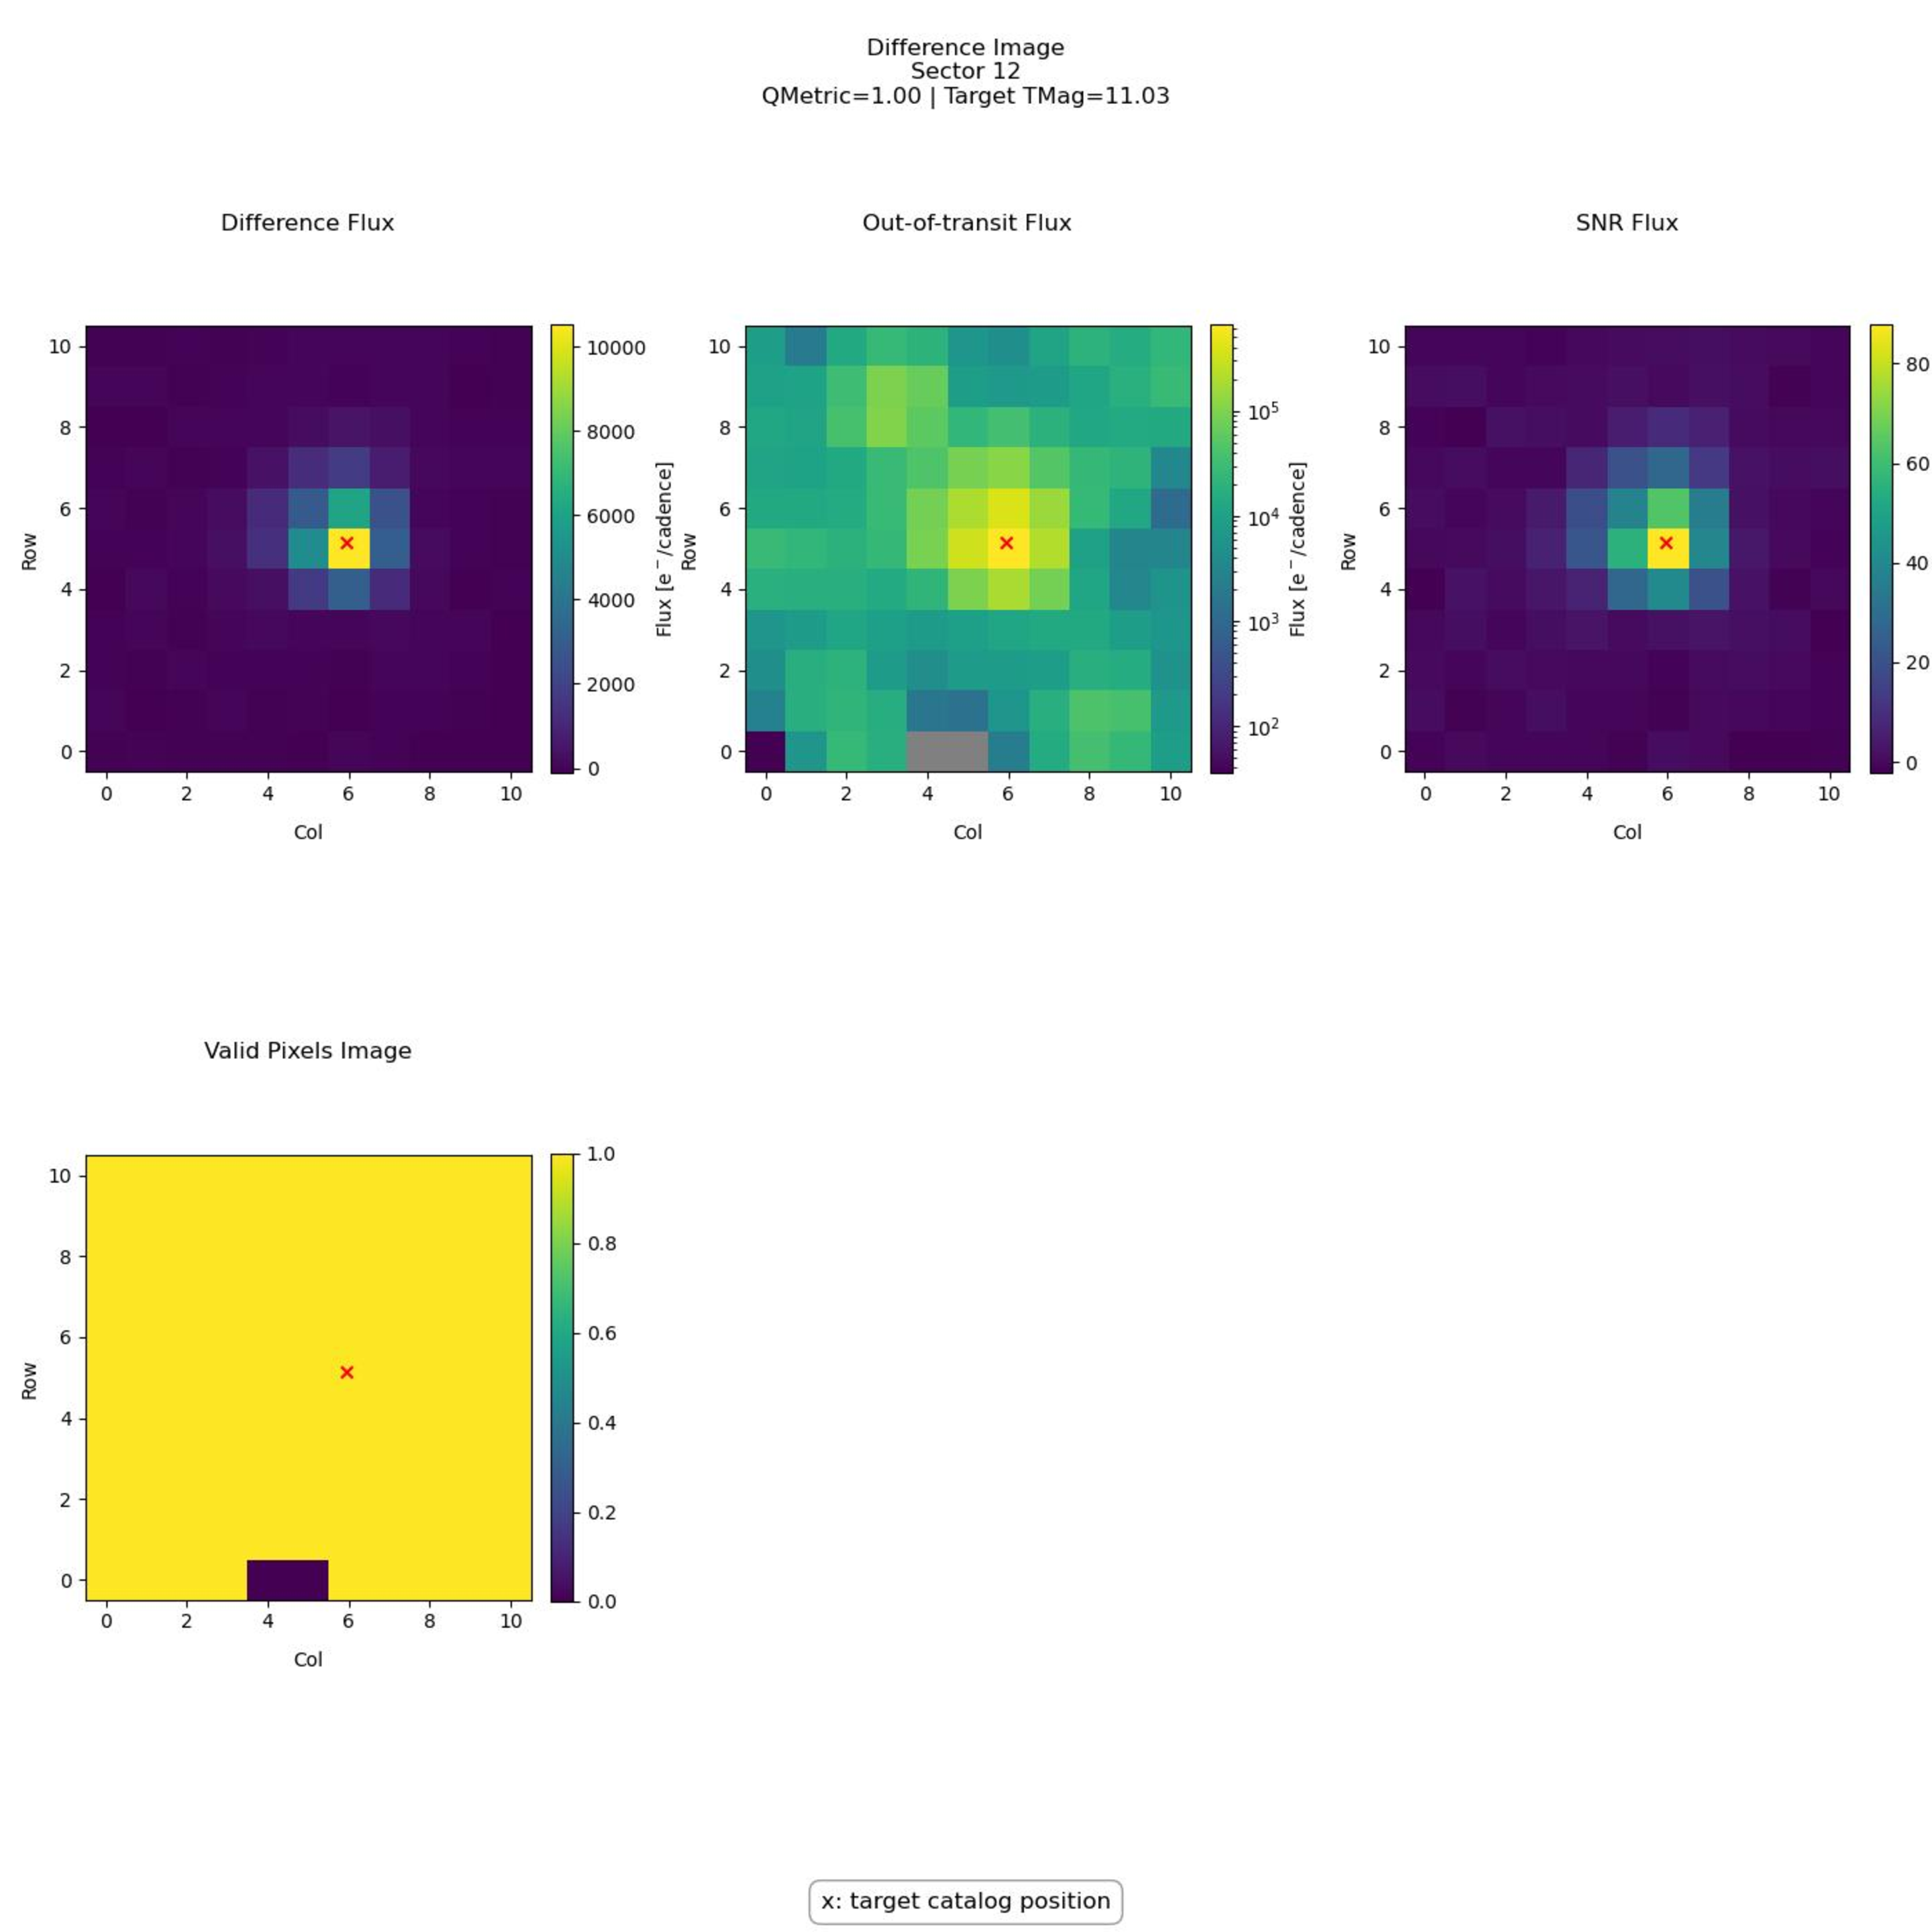
\includegraphics[width=\textwidth]{images/tess-spoc-tce_tic66818296-1-S1-92_summary_exominer-pipeline_diff-img.pdf}
    \caption{Difference image plots for \texttt{TIC 66818296.1} in sector 12.}
    \label{fig:diff_img}
\end{figure}

\section{Conclusion}

This document provides an overview of the outputs generated by the \ExoMinerPipeline. By producing both a detailed tabular prediction file and a visual diagnostic summary report, the pipeline serves as a tool for Subject Matter Experts (SMEs) engaged in the vetting and validation of exoplanet candidates from the TESS mission. The prediction table encapsulates crucial metadata, run provenance, and Machine Learning classification scores, while the auxiliary plots give SMEs insights into the data and the preprocessing steps taken to produce the data ingested by the model, as well as a better understanding of the model behavior and, ultimately, its prediction scores.

Any updates to the \ExoMinerPipeline\ and its outputs will be reflected in future versions of this document.

\section*{Acknowledgments}

The authors are supported through TESS XRP 2022 contract 22-XRP22\_2-0173, NASA Academic Mission Services (NAMS) contract number NNA16BD14C as well as the Intelligent Systems Research and Development Support-3 (ISRDS-3) Contract 80ARC020D00100. The SPOC collaborators are supported through NASA Cooperative Agreement 80NSSC21M0079.

Resources supporting this work were provided by the NASA High-End Computing (HEC) Program through the NASA Advanced Supercomputing (NAS) Division at Ames Research Center for the production of the Kepler SOC and the TESS SPOC data products and for training our deep learning model and preprocessing the data to be ingested by the model. 

Funding for the TESS mission is provided by NASA's Science Mission Directorate. This paper made use of data collected by the TESS mission and are publicly available from the Mikulski Archive for Space Telescopes (MAST) operated by the Space Telescope Science Institute (STScI). We acknowledge the use of public TESS data from pipelines at the TESS Science Office and at the TESS Science Processing Operations Center. This research has made use of the Exoplanet Follow-up Observation Program (ExoFOP; DOI: 10.26134/ExoFOP5) website, which is operated by the California Institute of Technology, under contract with the National Aeronautics and Space Administration under the Exoplanet Exploration Program. We would like to thank ExoFOP-TESS for hosting and sharing vetted TOI information and follow-up results, and the TESS Science Office and the TFOP SG1 Working Group, led by Dr. Karen A. Collins (CfA/SAO), for their vetting and ground-based follow-up of TESS Objects of Interest.

This material is based upon work supported by the NASA under Agreement No.\ 80NSSC21K0593 for the program ``Alien Earths''. The results reported herein benefited from collaborations and/or information exchange within NASA’s Nexus for Exoplanet System Science (NExSS) research coordination network sponsored by NASA’s Science Mission Directorate.

% We would also like to acknowledge the use of Microsoft Enterprise Copilot~\citep{microsoft2025copilot}, an AI-powered writing assistant, in editing portions of this manuscript to improve clarity and writing quality.

\printbibliography[heading=bibintoc]

\end{document}
